\documentclass{beamer}

\usepackage[T1]{fontenc}
\usepackage[utf8]{inputenc}
\usepackage[english]{babel}
\usepackage{lmodern}
\usepackage{tikz}
\usetikzlibrary{positioning}

% ----------------------------------------
%  ENVIRONMENT SETUP
% ----------------------------------------

\newenvironment{secframe}
  {\begin{frame}{\insertsection}} % ouverture : crée une frame avec le titre de la section courante
  {\end{frame}} 

% ----------------------------------------


% Use Unipd as theme, with options:
% - pageofpages: define the separation symbol of the footer page of pages (e.g.: of, di, /, default: of)
% - logo: position another logo near the Unipd logo in the title page (e.g. department logo), passing the second logo path as option 
% Use the environment lastframe to add the endframe text
\usetheme[pageofpages=of]{Unipd}

\title{I - Neural Turing Machines}
\subtitle{Application to physical simulations}
\author[Lucia Fernandez Sanchez, Alexandra Perruchot-Triboulet Rodriguez, Samuel Chapuis]{L.~Fernandez Sanchez \and A.~Perruchot-Triboulet Rodriguez \and S.~Chapuis}

\date{\today}

% The next block of commands puts the table of contents at the beginning of each section and highlights the current section
\AtBeginSection[]
{
  \begin{frame}
    \frametitle{Table of Contents}
    \tableofcontents[currentsection]
  \end{frame}
}



\begin{document}

% Make the title page
\frame{\titlepage}
\section{Foundations: The Navier--Stokes Equations}

% ===== Slide 1 =====
\begin{frame}{The Navier--Stokes Equations}
\small
% \textcolor{red_unipd}{\Large Neural PDE Modeling and Navier--Stokes Foundations}

\vspace{0.6em}

\begin{block}{Context}
The three main neural architectures studied in this project —  
\textbf{PINNs} (Raissi et al., 2017), \textbf{FNOs} (Li et al., 2020),  
and \textbf{NFTM} (Malhotra \& Seghouani, 2025) —  
all aim to approximate or emulate the behavior of \textbf{partial differential equations (PDEs)} derived from the \textbf{Navier–Stokes equations}.  

They differ in how they integrate physics:
\begin{itemize}
  \item \textbf{PINNs:} enforce the PDE directly in the loss function (physics-informed training);
  \item \textbf{FNOs:} learn an operator mapping between states of the PDE in Fourier space;
  \item \textbf{NFTM:} iteratively refines a learned physical field through neural “heads” and a controller.
\end{itemize}
All three trace back to the same physical foundation — the dynamics of fluids governed by Navier–Stokes.
\end{block}
\end{frame}




% ===== Slide 2 (Full Navier–Stokes) =====
\begin{frame}{The Navier--Stokes Equations}
\small
\textcolor{red_unipd}{\Large General Form of Navier--Stokes Equations}

\vspace{0.6em}

\begin{alertblock}{Equations}
\[
\begin{cases}
\dfrac{\partial \rho}{\partial t}
+ \nabla\!\cdot\!(\rho \mathbf{u}) = 0,\\[16pt]

\dfrac{\partial (\rho \mathbf{u})}{\partial t}
+ \nabla\!\cdot\!(\rho \mathbf{u} \otimes \mathbf{u})
= -\nabla p + \nabla\!\cdot\!\boldsymbol{\Sigma} + \rho \mathbf{g},\\[16pt]

\dfrac{\partial E}{\partial t}
+ \nabla\!\cdot\!((E+p)\mathbf{u})
= \nabla\!\cdot\!(\boldsymbol{\tau}\!\cdot\!\mathbf{u})
- \nabla\!\cdot\!\mathbf{q} + \rho \mathbf{u}\!\cdot\!\mathbf{g}
\end{cases}
\]
\end{alertblock}

\end{frame}




% ===== New Slide 3: Physical Meaning -- Mass Conservation =====
\begin{frame}{The Navier--Stokes Equations}
\small
\textcolor{red_unipd}{\Large Conservation Laws: Mass}

\vspace{0.8em}

\begin{alertblock}{Continuity equation -- Mass Conservation}
\[
\dfrac{\partial \rho}{\partial t} + \nabla\!\cdot\!(\rho \mathbf{u}) = 0
\]
\end{alertblock}

\begin{block}{Term definitions}
\begin{itemize}
  \item \(\rho\): fluid density \([\text{kg·m}^{-3}]\)
  \item \(\mathbf{u} = (u,v,w)\): velocity field \([\text{m·s}^{-1}]\)
  \item \(\nabla\!\cdot\!(\rho \mathbf{u})\): divergence of mass flux
  \item \(\partial \rho / \partial t\): local time rate of change of density
\end{itemize}
\end{block}
\end{frame}




% ===== Slide 4: Physical Meaning -- Momentum Conservation =====
\begin{frame}{The Navier--Stokes Equations}
\small
\textcolor{red_unipd}{\Large Conservation Laws: Momentum}

\vspace{0.8em}

\begin{alertblock}{Newton’s second law -- Momentum equation}
\[
\dfrac{\partial (\rho \mathbf{u})}{\partial t}
+ \nabla\!\cdot\!(\rho \mathbf{u}\otimes\mathbf{u})
= -\nabla p + \nabla\!\cdot\!\boldsymbol{\Sigma} + \rho \mathbf{g}
\]
\end{alertblock}

\begin{block}{Term definitions}
\begin{itemize}
  \item \(\rho \mathbf{u}\): momentum density \([\text{kg·m}^{-2}\text{·s}^{-1}]\)
  \item \(\nabla\!\cdot\!(\rho \mathbf{u}\otimes\mathbf{u})\): convective momentum transport
  \item \(-\nabla p\): pressure gradient force per unit volume
  \item \(\boldsymbol{\Sigma}\): viscous stress tensor \([\text{Pa}]\)
  \item \(\rho \mathbf{g}\): body force density (e.g. gravity) \([\text{N·m}^{-3}]\)
\end{itemize}
\end{block}
\end{frame}




% ===== Slide 5: Physical Meaning -- Energy Conservation =====
\begin{frame}{The Navier--Stokes Equations}
\small
\textcolor{red_unipd}{\Large Conservation Laws: Energy}

\vspace{0.8em}

\begin{alertblock}{Energy equation (first law of thermodynamics)}
\[
\dfrac{\partial E}{\partial t}
+ \nabla\!\cdot\!((E+p)\mathbf{u})
= \nabla\!\cdot\!(\boldsymbol{\tau}\!\cdot\!\mathbf{u})
- \nabla\!\cdot\!\mathbf{q}
+ \rho \mathbf{u}\!\cdot\!\mathbf{g}
\]
\end{alertblock}

\begin{block}{Term definitions}
\begin{itemize}
  \item \(E = \rho\!\left(e + \tfrac{1}{2}|\mathbf{u}|^2\right)\): total energy density (internal + kinetic)
  \item \(p\): pressure \([\text{Pa}]\)
  \item \(\boldsymbol{\tau}\): stress tensor (viscous + pressure)
  \item \(\mathbf{q}\): heat flux vector \([\text{W·m}^{-2}]\)
  \item \(\rho \mathbf{u}\!\cdot\!\mathbf{g}\): work done by body forces
\end{itemize}
\end{block}
\end{frame}




% ===== Slide 6 =====
\begin{frame}{The Navier--Stokes Equations}
\small
\textcolor{red_unipd}{\Large Newtonian Hypotheses and Constitutive Relations}

\begin{alertblock}{Viscous Stress}
\[
\begin{cases}
\boldsymbol{\Sigma} = \mu\left(\nabla \mathbf{u} + (\nabla \mathbf{u})^T\right) + \lambda (\nabla\!\cdot\!\mathbf{u}) \mathbf{I},\\[4pt]
\boldsymbol{\tau} = \boldsymbol{\Sigma} - p \mathbf{I}
\end{cases}
\]
\end{alertblock}

\begin{alertblock}{Heat Flux}
\[
\mathbf{q} = -k \nabla T
\]
\end{alertblock}

\begin{alertblock}{Internal Energy}
\[
E = \rho\left(e + \dfrac{1}{2}|\mathbf{u}|^2\right)
\]
\end{alertblock}

\end{frame}




% ===== Slide 7 (Navier–Stokes with Constitutive Relations Expanded) =====
\begin{frame}{The Navier--Stokes Equations}
\small
\textcolor{red_unipd}{\Large General Form with Constitutive Relations Expanded}

\vspace{0.6em}

\begin{alertblock}{Equations (Newtonian, compressible, viscous fluid)}
\[
\begin{cases}
\dfrac{\partial \rho}{\partial t}
+ \nabla\!\cdot\!(\rho \mathbf{u}) = 0,\\[16pt]

\rho\!\left(
\dfrac{\partial \mathbf{u}}{\partial t}
+ (\mathbf{u}\!\cdot\!\nabla)\mathbf{u}
\right)
= -\nabla p
+ \nabla\!\cdot\!\Big[
\mu\!\left(\nabla \mathbf{u} + (\nabla \mathbf{u})^T\right)
+ \lambda (\nabla\!\cdot\!\mathbf{u})\mathbf{I}
\Big]
+ \rho \mathbf{g},\\[20pt]

\dfrac{\partial }{\partial t}\!
\left[\rho\!\left(e + \dfrac{1}{2}|\mathbf{u}|^2\right)\right]
+ \nabla\!\cdot\!
\left[\rho\!\left(e + \dfrac{1}{2}|\mathbf{u}|^2\right)\mathbf{u} + p\mathbf{u}\right]
= \\ \nabla\!\cdot\!
\Big\{
\mu\!\left(\nabla \mathbf{u} + (\nabla \mathbf{u})^T\right)\!\cdot\!\mathbf{u}
+ \lambda (\nabla\!\cdot\!\mathbf{u})\mathbf{u}
- k\nabla T
\Big\}
+ \rho \mathbf{u}\!\cdot\!\mathbf{g}
\end{cases}
\]
\end{alertblock}

\end{frame}




% ===== Slide 8 =====
\begin{frame}{The Navier--Stokes Equations}
\small
\textcolor{red_unipd}{\Large Why Navier--Stokes Matters in Neural PDEs}

\vspace{0.6em}

\begin{block}{Central role in neural modeling}
The Navier--Stokes system unifies diffusion (viscous term),  
advection (nonlinear term), and incompressibility (constraint).  
Each paper tests neural architectures by simplifying or approximating parts of this system:
\begin{itemize}
  \item \textbf{PINNs:} direct enforcement of differential operators;
  \item \textbf{FNOs:} operator learning across time steps of Navier–Stokes;
  \item \textbf{NFTM:} learned iterative refinement mimicking PDE rollouts.
\end{itemize}
\vspace{0.4em}
Through these methods, the goal is to determine whether deep neural architectures can reproduce  
\textit{the stability and accuracy of physical solvers} for complex spatio-temporal dynamics.
\end{block}
\end{frame}

\section{From Navier--Stokes to Simplified PDEs}

% ===== Slide 1 =====
\begin{frame}{Navier Stokes to Simplified PDEs}
\small
\textcolor{red_unipd}{\Large Navier--Stokes (2D, incompressible)}

\vspace{0.6em}

\begin{alertblock}{Equation}
\[
\begin{cases}
\dfrac{\partial \mathbf{u}}{\partial t} 
+ (\mathbf{u}\!\cdot\!\nabla)\mathbf{u}
= -\nabla p + \nu\nabla^2 \mathbf{u},\\[4pt]
\nabla\!\cdot\!\mathbf{u} = 0
\end{cases}
\]
\end{alertblock}

\vfill

\begin{block}{Hypotheses}
Incompressible: \(\nabla\!\cdot\!\mathbf{u} = 0\). \quad
Viscous: \(\nu>0\). \quad
Free pressure: \(p(x,y,t)\).
\end{block}
\end{frame}


% ===== Slide 2 =====
\begin{frame}{Navier Stokes to Simplified PDEs}
\small
\textcolor{red_unipd}{\Large Euler (Inviscid Fluid)}

\vspace{0.6em}

\begin{alertblock}{Equation}
\[
\dfrac{\partial \mathbf{u}}{\partial t} 
+ (\mathbf{u}\!\cdot\!\nabla)\mathbf{u}
= -\nabla p
\]
\end{alertblock}

\vfill

\begin{block}{Hypotheses}
No viscosity: \(\nu = 0\). \quad
(Optional) Incompressible: \(\nabla\!\cdot\!\mathbf{u}=0\).
\end{block}
\end{frame}


% ===== Slide 3 =====
\begin{frame}{Navier Stokes to Simplified PDEs}
\small
\textcolor{red_unipd}{\Large Burgers (1D Advection–Diffusion)}

\vspace{0.6em}

\begin{alertblock}{Equation}
\[
\dfrac{\partial u}{\partial t} + u\dfrac{\partial u}{\partial x}
= \nu\dfrac{\partial^2 u}{\partial x^2}
\]
\end{alertblock}

\vfill

\begin{block}{Hypotheses}
\(\nabla p=\mathbf{0}\). \quad
1D reduction: \(\mathbf{u}=(u(x,t),0)\). \quad
Self-advection: \(u\,\partial_x u\).
\end{block}
\end{frame}


% ===== Slide 4 =====
\begin{frame}{Navier Stokes to Simplified PDEs}
\small
\textcolor{red_unipd}{\Large Heat / Diffusion Equation}

\vspace{0.6em}

\begin{alertblock}{Equation}
\[
\dfrac{\partial u}{\partial t} =
\alpha\,\dfrac{\partial^2 u}{\partial x^2}
\]
\end{alertblock}

\vfill

\begin{block}{Hypotheses}
No convection: \(u\,\partial_x u = 0\). \quad
Pure diffusion: \(\alpha>0\).
\end{block}
\end{frame}


% ===== Slide 5 =====
\begin{frame}{Navier Stokes to Simplified PDEs}
\small
\textcolor{red_unipd}{\Large Darcy (Steady, Elliptic Form)}

\vspace{0.6em}

\begin{alertblock}{Equation}
\[
\nabla\!\cdot\!\big(a(x)\nabla u(x)\big) = f(x)
\]
\end{alertblock}

\vfill

\begin{block}{Hypotheses}
Steady regime: \(\partial_t u = 0\). \quad
Heterogeneous medium: \(a(x)>0\). \quad
Source/sink: \(f(x)\).
\end{block}
\end{frame}



% ===== Slide 6 =====
\begin{frame}{Navier Stokes to Simplified PDEs}
\small
\textcolor{red_unipd}{\Large Summary of Relationships}

\centering
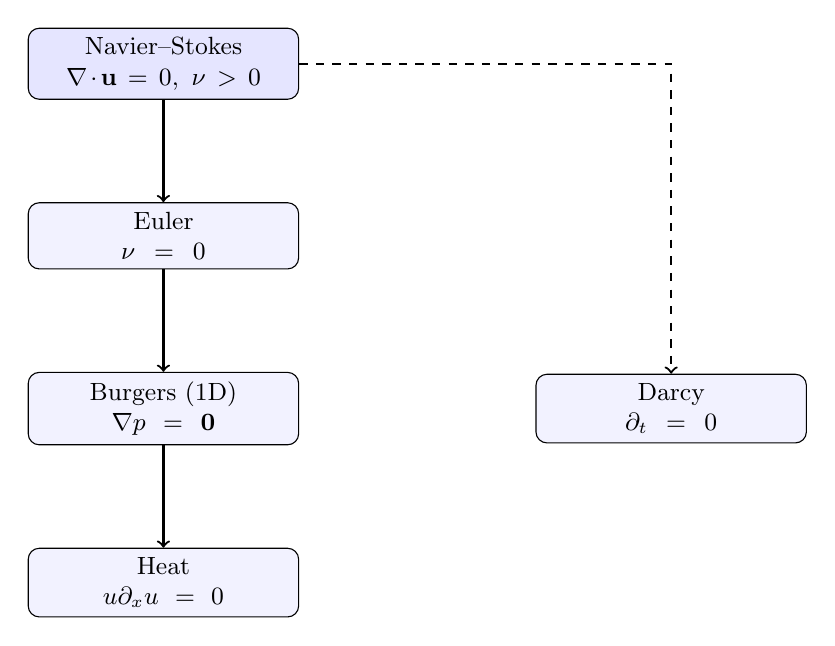
\begin{tikzpicture}[node distance=1.3cm, every node/.style={align=center, font=\small}]
\node (NS) [draw, rounded corners, fill=blue!10, text width=3.2cm] {Navier--Stokes \\ \(\nabla\!\cdot\!\mathbf{u}=0,\ \nu>0\)};
\node (E) [draw, rounded corners, below=of NS, fill=blue!5, text width=3.2cm] {Euler \\ \(\nu=0\)};
\node (B) [draw, rounded corners, below=of E, fill=blue!5, text width=3.2cm] {Burgers (1D) \\ \(\nabla p=\mathbf{0}\)};
\node (H) [draw, rounded corners, below=of B, fill=blue!5, text width=3.2cm] {Heat \\ \(u\partial_x u=0\)};
\node (D) [draw, rounded corners, right=3.0cm of B, fill=blue!5, text width=3.2cm] {Darcy \\ \(\partial_t=0\)};
\draw[->, thick] (NS) -- (E);
\draw[->, thick] (E) -- (B);
\draw[->, thick] (B) -- (H);
\draw[->, thick, dashed] (NS) -| (D);
\end{tikzpicture}
\end{frame}


\section{2D Burgers Equation}

\begin{secframe}
\small
\textcolor{red_unipd}{\Large Section Overview}

\begin{alertblock}{Goal}
    Compare a physical simulator and a Neural Field Turing Machine (NFTM) for solving the 2D Burgers equation.

\end{alertblock}

\begin{block}{Approach}
Build a numerical solver, then train and evaluate NFTM on the same problem.
\end{block}
\end{secframe}

% ===== Slide 1 =====
\begin{secframe}
\small
\textcolor{red_unipd}{\Large Governing Equations}

\vspace{0.6em}

\begin{alertblock}{Equation}
\[
\begin{cases}
  u_t + u u_x + v u_y = \nu (u_{xx} + u_{yy}), \\
  v_t + u v_x + v v_y = \nu (v_{xx} + v_{yy})
\end{cases}
\]
\end{alertblock}

\vfill

\begin{block}{Hypotheses}
\(\nabla p=\mathbf{0}\). \quad
1D reduction: \(\mathbf{u}=(u(x,t),0)\). \quad
Self-advection: \(u\,\partial_x u\).
\end{block}

\vspace{0.5em}

\begin{block}{Einstein notation}
$u_t = \frac{\partial u}{\partial t}$, $u_x = \frac{\partial u}{\partial x}$, $u_{xx} = \frac{\partial^2 u}{\partial x^2}$, etc.
\end{block}

\end{secframe}

% ===== Advection Frame =====
\begin{secframe}
\small
\textcolor{red_unipd}{\Large Advection}

\vspace{0.6em}

\begin{block}{Advection Terms}
\begin{itemize}
    \item \textbf{$u u_x$, $v v_y$, $u v_x$, $v u_y$}: Nonlinear advection terms.
    \item Represent transport of velocity due to the flow itself.
\end{itemize}
\end{block}

\begin{figure}[h]
    \centering
    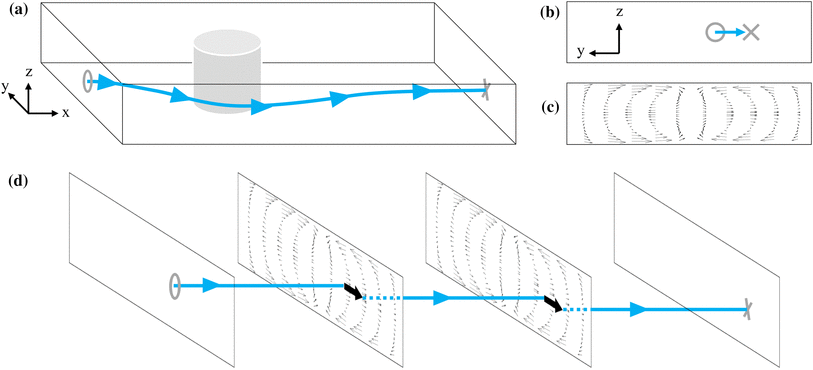
\includegraphics[width=0.7\linewidth]{images/advection.png}
\end{figure}

\end{frame}

% ===== Diffusion Frame =====
\begin{frame}{2D Burgers Equation}
\small
\textcolor{red_unipd}{\Large Diffusion}

\vspace{0.6em}

\begin{block}{Diffusion Terms}
\begin{itemize}
    \item \textbf{$\nu (u_{xx} + u_{yy})$, $\nu (v_{xx} + v_{yy})$}: Diffusion terms.
    \item Model the spreading and smoothing of velocity due to viscosity $\nu$.
\end{itemize}
\end{block}

\begin{figure}[h]
    \centering
    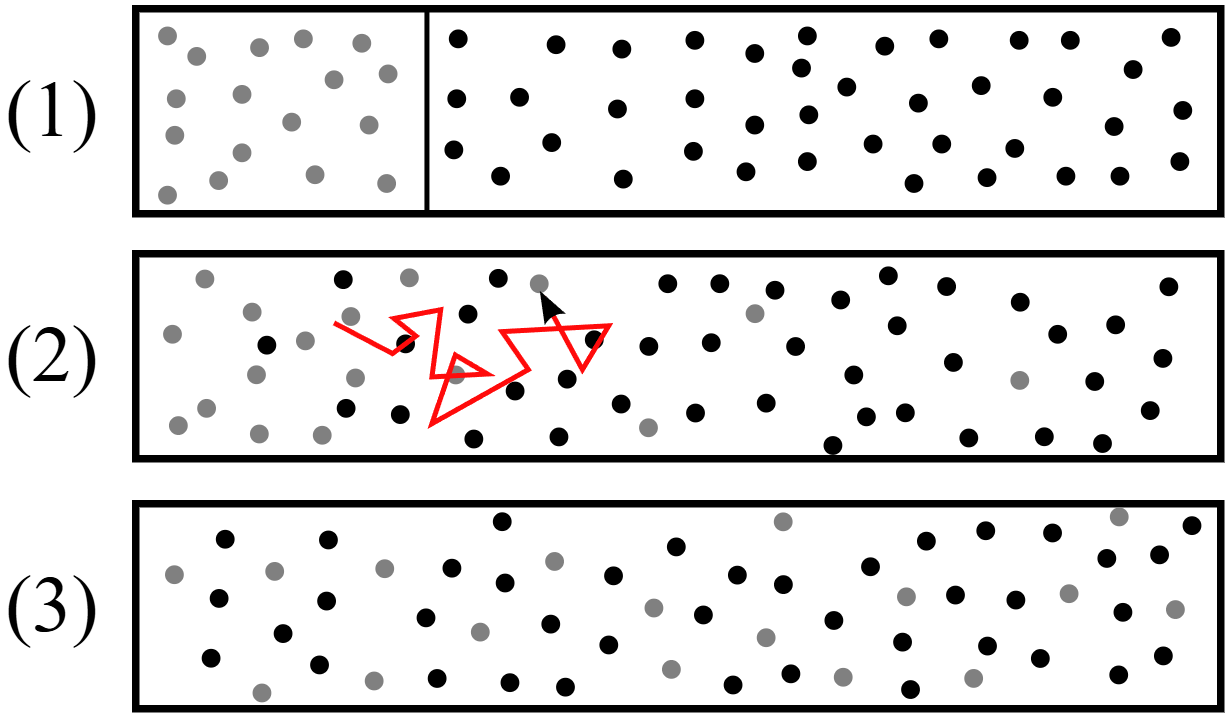
\includegraphics[width=0.7\linewidth]{images/diffusion.png}
\end{figure}


\end{secframe}

% ===== Balance Frame =====
\begin{secframe}
\small
\textcolor{red_unipd}{\Large Pressure gradient}

\vspace{0.6em}

\begin{alertblock}{Pressure Gradient Terms}
  The huge Hypotheses here is \(\nabla p=\mathbf{0}\), so there is no effect of the pressure in the equation. \\
  \( \Rightarrow \) Only the initial velocity has an influence on the evolution of the system
\end{alertblock}

\begin{example}
  Consider a scenario where the initial velocity is constant across the domain on airfoil shape. \\
  Since \(\nabla p=\mathbf{0}\), the pressure gradient does not influence the flow. \\
  The flow will not change over time, remaining constant as per the initial condition.
\end{example}



\end{secframe}

% ===== Slide 2 =====
\begin{secframe}
\small
\textcolor{red_unipd}{\Large Numerical Simulation}

\vspace{0.6em}

\begin{block}{Description}
\begin{itemize}
  \item Implements the PDE directly using finite difference methods.
  \item Discretizes space and time; updates velocity fields step by step.
  \item Parameters: grid size, time step, viscosity, initial/boundary conditions.
\end{itemize}
\end{block}

\begin{alertblock}{Finite Difference Schemes}
\begin{itemize}
  \item Forward difference (time): $u_t \approx \frac{u_{i,j}^{n+1} - u_{i,j}^n}{\Delta t}$
  \item Central difference (space): $u_x \approx \frac{u_{i+1,j}^n - u_{i-1,j}^n}{2\Delta x}$
  \item Central difference (second derivative): $u_{xx} \approx \frac{u_{i+1,j}^n - 2u_{i,j}^n + u_{i-1,j}^n}{\Delta x^2}$
\end{itemize}
\end{alertblock}

\end{secframe}

% ===== Slide 3 =====
\begin{secframe}
\small
\textcolor{red_unipd}{\Large Neural Field Turing Machine}

\vspace{0.6em}

\begin{alertblock}{Objective}
\begin{itemize}
  \item Learns to update field values using neural controllers and local memory patches.
  \item Trained on data from the physical simulator or existing datasets.
  \item Can generalize to new initial conditions or parameters.
\end{itemize}
\end{alertblock}

\begin{block}{Datasets}
\begin{itemize}
  \item Use existing benchmark datasets for PDEs (if available).
  \item Generate custom datasets using our physical simulator (varied initial/boundary conditions, parameters).
\end{itemize}
\end{block}
\end{secframe}


% ===== Slide 5 =====
\begin{secframe}
\small
\textcolor{red_unipd}{\Large Summary \& Next Steps}

\vspace{0.6em}

\begin{block}{Next Steps}
\begin{itemize}
  \item Build and validate the physical simulator.
  \item Train NFTM on generated and existing datasets.
  \item Compare performance, accuracy, and generalization.
\end{itemize}
\end{block}
\end{secframe}

% HAHAAHS


%%%%%%%%%%%%%%%%%%%%%%%%%%%%%%%%%%%%
% EXEMPLE SLIDES
%%%%%%%%%%%%%%%%%%%%%%%%%%%%%%%%%%%%

% \section{First section}

%     \begin{frame}{First section}
%         In this slide, some important text will be
%         \alert{highlighted} because it's important.
%         Here an ordered list:
%         \begin{enumerate}
%             \item First item
%             \item Second item
%         \end{enumerate}
%         Here an unordered list: 
%         \begin{itemize}
%             \item One item
%             \item Another item
%         \end{itemize}
%     \end{frame}
    
% \section{Second section}

%     \begin{frame}{Second section}
%         \begin{block}{Block}
%             Sample text in a normal block
%         \end{block}
   
%         \begin{alertblock}{Alert block}
%             Sample text in an alert block
%         \end{alertblock}    
        
%          \begin{example}
%             Sample text for an example
%         \end{example}
%     \end{frame}

    
%     \begin{emptyframe}
%         Thank you!
%     \end{emptyframe}

%     \appendix

%     \begin{frame}{Backup slide}
%         Some additional content
%     \end{frame}
    
\end{document}